\documentclass[12pt, a4paper, oneside]{ctexart}
\usepackage{amsmath, amsthm, amssymb, graphicx}
\usepackage[bookmarks=true, colorlinks, citecolor=blue, linkcolor=black]{hyperref}
\usepackage{listings}
\usepackage{xcolor}
\usepackage{inconsolata}
\usepackage{booktabs}
\usepackage{geometry}
\geometry{left=2cm, right=2cm} 
% 定义可能使用到的颜色
\definecolor{CPPLight}  {HTML} {686868}
\definecolor{CPPSteel}  {HTML} {888888}
\definecolor{CPPDark}   {HTML} {262626}
\definecolor{CPPBlue}   {HTML} {4172A3}
\definecolor{CPPGreen}  {HTML} {487818}
\definecolor{CPPBrown}  {HTML} {A07040}
\definecolor{CPPRed}    {HTML} {AD4D3A}
\definecolor{CPPViolet} {HTML} {7040A0}
\definecolor{CPPGray}  {HTML} {B8B8B8}
\lstset{basicstyle=\ttfamily,breaklines=true}
\lstset{
    columns=fixed,       
    numbers=left,                                        % 在左侧显示行号
    numbersep=5pt,
    frame=none,                                          % 不显示背景边框
    backgroundcolor=\color[RGB]{245,245,244},            % 设定背景颜色
    keywordstyle=\color[RGB]{40,40,255},                 % 设定关键字颜色
    numberstyle=\footnotesize\color{red},           % 设定行号格式
    commentstyle=\it\color[RGB]{0,96,96},                % 设置代码注释的格式
    stringstyle=\rmfamily\slshape\color[RGB]{128,0,0},   % 设置字符串格式
    showstringspaces=false,                              % 不显示字符串中的空格
    language=c,                                        % 设置语言
    xleftmargin=1em, %整体距左侧边线的距离为2em
    morekeywords={alignas,continute,friend,register,true,alignof,decltype,goto,
    reinterpret_cast,try,asm,defult,if,return,typedef,auto,delete,inline,short,
    typeid,bool,do,int,signed,typename,break,double,long,sizeof,union,case,
    dynamic_cast,mutable,static,unsigned,catch,else,namespace,static_assert,using,
    char,enum,new,static_cast,virtual,char16_t,char32_t,explict,noexcept,struct,
    void,export,nullptr,switch,volatile,class,extern,operator,template,wchar_t,
    const,false,private,this,while,constexpr,float,protected,thread_local,
    const_cast,for,public,throw,std},
}
% 导言区

\title{计算机系统基础 \\ Lab4 Cache Lab} % 标题
\author{姓名:傅文杰\\学号:22300240028} % 作者
\date{\today} % 日期

\begin{document}

\maketitle % 生成标题

\tableofcontents % 生成目录

\section{实验A:编写高速缓存} % 一级标题

\subsection{实验要求}
\noindent
在csim.c下编写一个高速缓存模拟器来对内存读写操作进行正确的反馈。\\这个模拟器有 6 个参数:
\begin{lstlisting}
Usage: ./csim-ref [-hv] -s <s> -E <E> -b <b> -t <tracefile>
\end{lstlisting}
\subsubsection{参数说明}
\begin{itemize}
    \item -h: Optional help flag that prints usage info
    \item -v: Optional verbose flag that displays trace info
    \item -s $<$s$>$: Number of set index bits (S = $2^s$ is the number of sets)
    \item -E $<$E$>$: Associativity (number of lines per set)
    \item -b $<$b$>$: Number of block bits (B = $2^b$ is the block size)
    \item -t $<$tracefile$>$: Name of the valgrind trace to replay    
\end{itemize}
对于-v参数,我们需要初始化一个标记。
\begin{lstlisting}
int verbose = 0; 
\end{lstlisting}
对于文件当中对于缓存的操作,也就是-t参数读入的文件,我们需要初始化一个数组保存其中的内容。
\begin{lstlisting}
char t[1000];
\end{lstlisting}
\subsubsection{trace格式说明}
\noindent
输入的 trace 的格式为:空格 + operation address + , + size\\
operation 有 4 种:
\begin{itemize}
    \item I 加载指令
    \item L 加载数据
    \item S 存储数据 
    \item M 修改数据
\end{itemize}

\subsubsection{模拟器反馈说明}
\noindent
模拟器不需要考虑加载指令,而M指令就相当于先进行L再进行S。\\
模拟器要做出的反馈有 3 种:
\begin{itemize}
    \item hit:命中,表示要操作的数据在对应组的其中一行
    \item miss:不命中,表示要操作的数据不在对应组的任何一行
    \item eviction:驱赶,表示要操作的数据的对应组已满,进行了替换操作
\end{itemize}
因此我们要初始化这些信息
\begin{lstlisting}
int hit_count = 0, miss_count = 0, eviction_count = 0; 
\end{lstlisting}
最后打印出来
\begin{lstlisting}
printSummary(hit_count, miss_count, eviction_count);
\end{lstlisting}
\subsection{实验准备}
\subsubsection{头文件}
\noindent
由于我们不是shark machine,所以为了调用getopt函数
我们需要引入头文件unistd.h和getopt.h
\subsubsection{替换策略}
\noindent
缓存不命中时,CPU必须从内存中取出包含这个字的块,并替换一行。
书上有两个策略:
\begin{itemize}
    \item LFU:替换在过去某个时间窗口内引用次数最少的一行
    \item LRU:替换最后一次访问时间最久远的一行
\end{itemize}
Hints提示我们使用LRU counter计数器,即时间戳。除此以外,还可以
使用链表,哈希表加双向链表等复杂数据结构来实现。这里选择较为简单的时间戳方法。
\subsubsection{Cache的结构}
\noindent
\begin{figure}[htbp]
    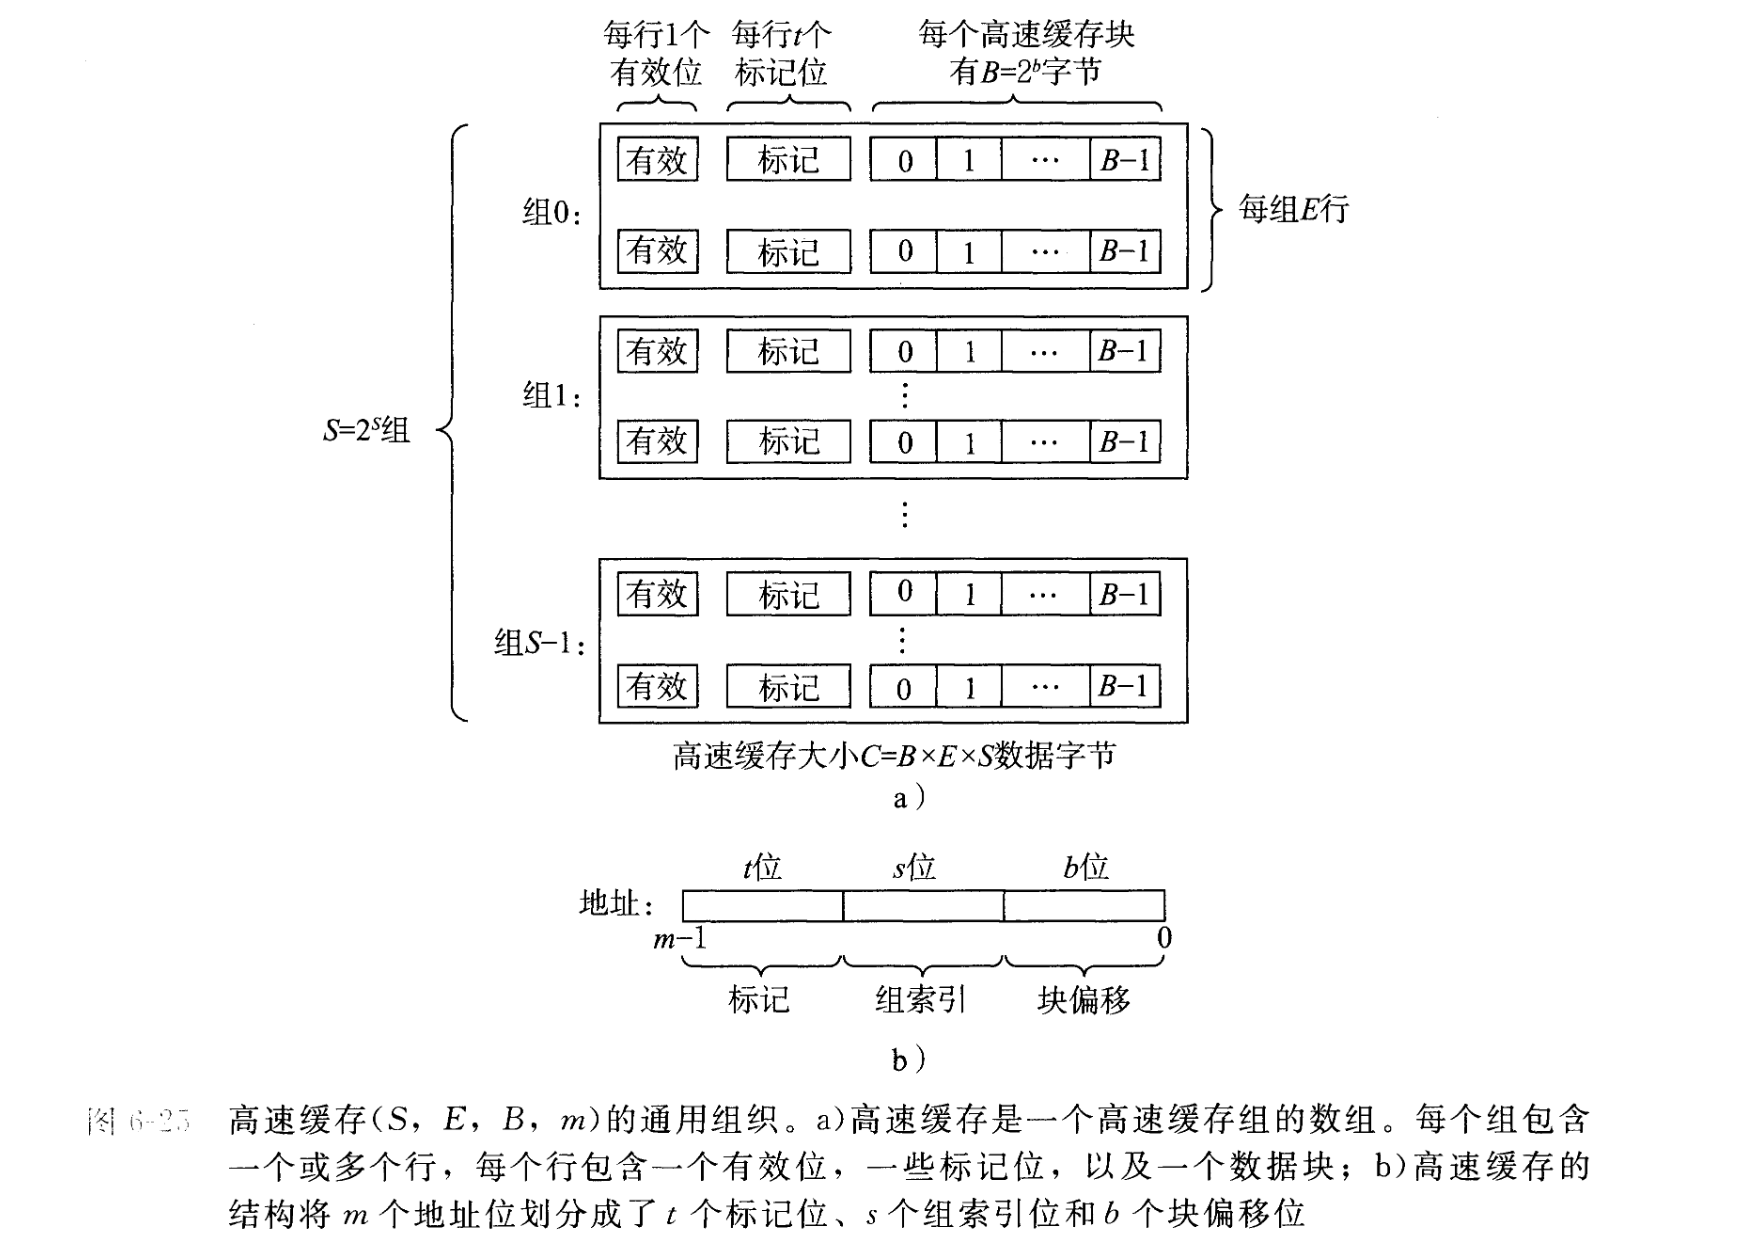
\includegraphics[scale=0.31]{image/1-1.png}
\end{figure}
对于整个缓存,我们需要定义两个结构体,cache\_ 和 cache\_line。\\
其中cache\_对应的是整个缓存$(S, E, B, m)$的通用组织,由于
$M=2^m$代表总的地址数目,可以由其他变量计算出,因此可以省略。
\begin{lstlisting}
typedef struct cache_
{
    int S;
    int E;
    int B;
    Cache_line **line;
} Cache;
Cache *cache = NULL;
\end{lstlisting}
cache\_line对应的是缓存中的行的信息,除了有效位和标记外,还需要LRU方法的时间戳。
\begin{lstlisting}
typedef struct cache_line
{
    int valid;     
    int tag;       
    int time_tamp; 
} Cache_line;
\end{lstlisting}
\subsection{主函数}
\noindent
由1.1.1可知我们需要接受6个参数,可以参考如下的example。\\
\begin{figure}[htbp]
    \centering
    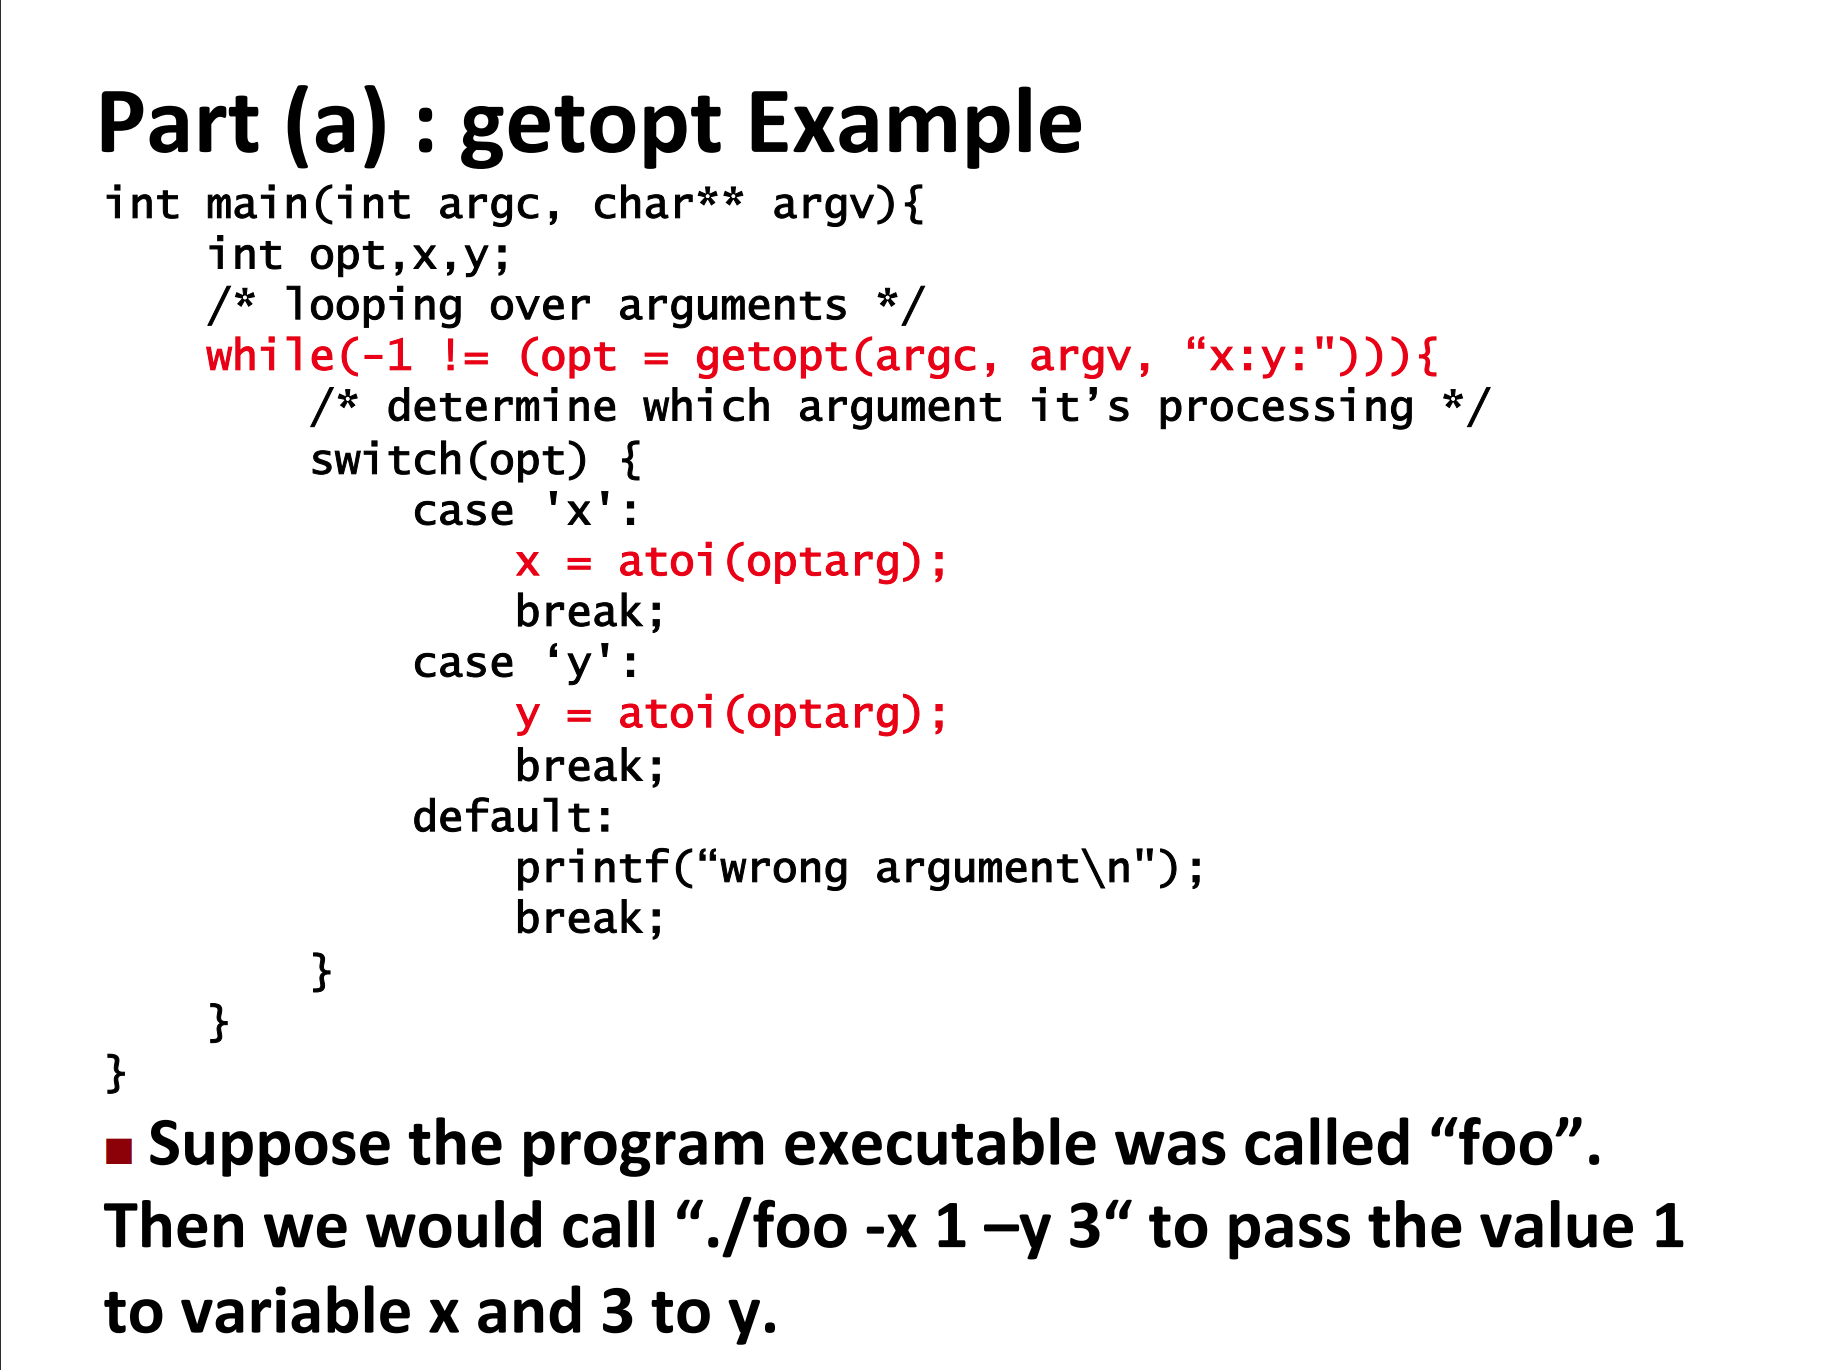
\includegraphics[scale=0.2]{image/2-1.png}
\end{figure}
我们的局部变量为:opt(设置成char类型), $s(S = 2^s $是组的个数$), E($是行数$), b(B = 2^b $是每个缓冲块的字节数$)$。\\
我们需要定义的函数为:
\begin{enumerate}
    \item 打印帮助:print\_help函数
    \item Cache操作:Init\_Cache初始化缓存,get\_trace读取trace中的操作,free\_Cache释放缓存
\end{enumerate}
代码如下:
\begin{lstlisting}
int main(int argc, char *argv[])
{
    char opt;
    int s, E, b;
    while (-1 != (opt = getopt(argc, argv, "hvs:E:b:t:")))
    {
        switch (opt)
        {
        case 'h':
            print_help();
            exit(0);
        case 'v':
            verbose = 1;
            break;
        case 's':
            s = atoi(optarg);
            break;
        case 'E':
            E = atoi(optarg);
            break;
        case 'b':
            b = atoi(optarg);
            break;
        case 't':
            strcpy(t, optarg);
            break;
        default:
            print_help();
            exit(-1);
        }
    }
    Init_Cache(s, E, b);
    get_trace(s, E, b);
    free_Cache();
    printSummary(hit_count, miss_count, eviction_count);
    return 0;
}
\end{lstlisting}
\subsection{Cache相关函数}
\subsubsection{初始化}
\noindent
初始化$S=2^s$组数,$E$每组E行,$B=2^b$每个告诉缓存块的字节数;\\
为Cache分配空间,并产生一个指向它的指针(Cache* cache);\\
为cache的二维数组分配空间(S组一维cache\_line),每个一维cache\_line数组有E个cache\_line;\\
每个cache\_ling的有效位、标记、时间戳分别初始化为0, -1, 0。
代码如下:
\begin{lstlisting}
void Init_Cache(int s, int E, int b)
{
    int S = 1 << s;
    int B = 1 << b;
    cache = (Cache *)malloc(sizeof(Cache));
    cache->S = S;
    cache->E = E;
    cache->B = B;
    cache->line = (Cache_line **)malloc(sizeof(Cache_line *) * S);
    for (int i = 0; i < S; i++)
    {
        cache->line[i] = (Cache_line *)malloc(sizeof(Cache_line) * E);
        for (int j = 0; j < E; j++)
        {
            cache->line[i][j].valid = 0; 
            cache->line[i][j].tag = -1;
            cache->line[i][j].time_tamp = 0;
        }
    }
}
\end{lstlisting}
\subsubsection{释放空间}
\noindent
每次malloc分配空间之后一定要释放空间。
我们在初始化的时候为缓存、缓存的每个组、每个组的每行分配了空间,需要对应地释放掉。\\
代码如下:
\begin{lstlisting}
void free_Cache()
{
    int S = cache->S;
    for (int i = 0; i < S; i++)
    {
        free(cache->line[i]);
    }
    free(cache->line);
    free(cache);
}
\end{lstlisting}
\subsubsection{缓存操作}
\noindent
由1.1.3,对于缓存的操作,我们只需要实现读操作和写操作就能完成所有的操作。
但其实读操作就相当于“不写”的写操作,我们可以把它们统一为更新操作。
除此之外,我们还需要想办法得到输入的标记位和组序号。
因此代码大致架构如下:
\begin{lstlisting}
void get_trace(int s, int E, int b)
{
    FILE *pFile;
    pFile = fopen(t, "r");
    if (pFile == NULL)
    {
        exit(-1);
    }
    char identifier;
    unsigned address;
    int size;
    // Reading lines like " M 20,1" or "L 19,3"
    while (fscanf(pFile, " %c %x,%d", &identifier, &address, &size) > 0)
    {
        int op_tag = ...;
        int op_s = ...;
        switch (identifier)
        {
        case 'M': 
            update_info(op_tag, op_s);
            update_info(op_tag, op_s);
            break;
        case 'L':
            update_info(op_tag, op_s);
            break;
        case 'S':
            update_info(op_tag, op_s);
            break;
        }
    }
    fclose(pFile);
}
\end{lstlisting}
首先,由第4页上地址的图示,我们可以通过位运算得到标记和组索引。\\
将地址右移(s+b)位就得到标记(C语言算术右移)。\\
将地址右移b位,再和$0x\underbrace{0 \cdots 0}_{(64-s)bits}\underbrace{1 \cdots 1}_{(s) bits}$相与即可。\\
代码如下:
\begin{lstlisting}
int op_tag = address >> (s + b);
int op_s = (address >> b) & ((unsigned)(-1) >> (64 - s));
\end{lstlisting}
更新操作:如果有效位设置了并且tag符合,那么命中,否则不命中。\\
\begin{figure}[hbtp]
    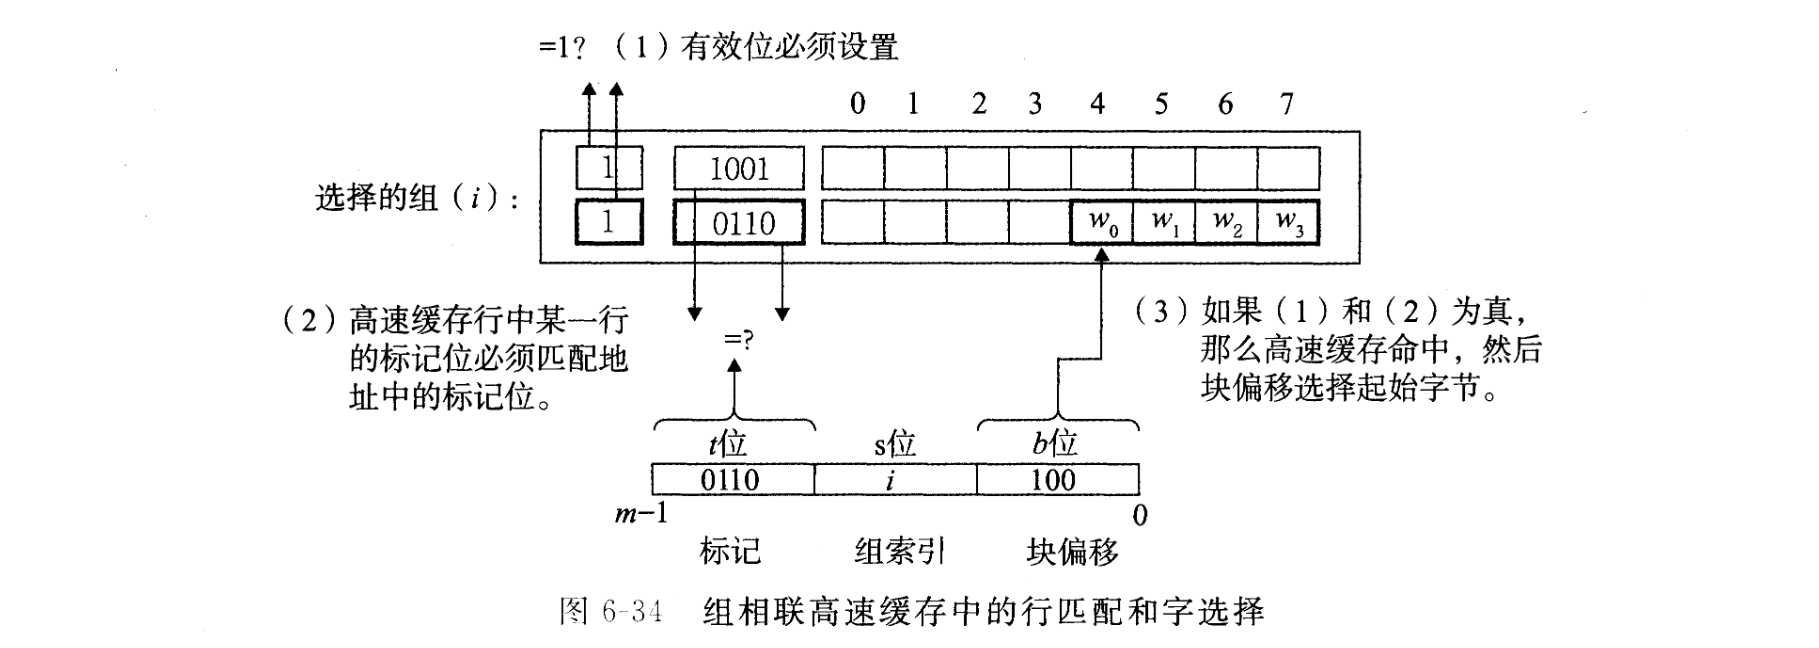
\includegraphics[scale=0.4]{image/2-3.png}
\end{figure}
不命中时:如果有空行,那么缓存需要从内存中取出这个块并替换空行,否则,即cache\_line满了,
我们需要找到时间戳最大的行,并替换。\\
最后要记得更新:如果命中,需要更新时间戳,如果没有命中,需要把有效位设置为1,把标记位设置为从内存中读的tag,并更新时间戳。\\
时间戳的更新方法为:对于操作的缓存行,时间戳更新为0,对于没有操作的缓存行,时间戳++。注意更新时间戳的前提是有效位为1。\\
代码如下:
\begin{lstlisting}
void update(int i, int op_s, int op_tag)
{
    cache->line[op_s][i].valid=1;
    cache->line[op_s][i].tag = op_tag;
    for(int k = 0; k < cache->E; k++)
        if(cache->line[op_s][k].valid==1)
            cache->line[op_s][k].time_tamp++;
    cache->line[op_s][i].time_tamp = 0;
}
int find_LRU(int op_s)
{
    int max_index = 0;
    int max_stamp = 0;
    for(int i = 0; i < cache->E; i++){
        if(cache->line[op_s][i].time_tamp > max_stamp){
            max_stamp = cache->line[op_s][i].time_tamp;
            max_index = i;
        }
    }
    return max_index;
}
int is_full(int op_s)
{
    for (int i = 0; i < cache->E; i++)
    {
        if (cache->line[op_s][i].valid == 0)
            return i;
    }
    return -1;
}
int get_index(int op_s, int op_tag)
{
    for (int i = 0; i < cache->E; i++)
    {
        if (cache->line[op_s][i].valid && cache->line[op_s][i].tag == op_tag)
            return i;
    }
    return -1;
}
void update_info(int op_tag, int op_s)
{
    int index = get_index(op_s, op_tag);
    if (index == -1)
    {
        miss_count++;
        if (verbose)
            printf("miss ");
        int i = is_full(op_s);
        if(i==-1){
            eviction_count++;
            if(verbose) printf("eviction");
            i = find_LRU(op_s);
        }
        update(i,op_s,op_tag);
    }
    else{
        hit_count++;
        if(verbose)
            printf("hit");
        update(index,op_s,op_tag);    
    }
}
\end{lstlisting}
\section{实验B:优化矩阵转置}
\subsection{实验要求}
\noindent
在trans.c中写转置函数使得cache miss尽可能少。
\begin{itemize}
    \item $32 \times 32$ 的矩阵需要使miss次数小于300
    \item $64 \times 64$ 的矩阵需要使miss次数小于1300
    \item $61 \times 67$ 的矩阵需要使miss次数小于2000
\end{itemize}
这里的缓存参数为$(s = 5, E = 1, b = 5)$,即$S = 2^s = 2^5 = 32$个CacheLine、每个CacheLine有$E=1$组、每组可以存储$B = 2^b = 2^5 = 32$个Byte($8 \times sizeof(int)$)。\\
如果我们用直接的暴力矩阵转置:
\begin{lstlisting}
void trans_submit(int M, int N, int A[N][M], int B[M][N]) {
    for (int i = 0; i < N; i++) {
        for (int j = 0; j < M; j++) {
            int tmp = A[i][j];
            B[j][i] = tmp;
        }
    }
}
\end{lstlisting}
在终端中运行测试:
\begin{lstlisting}
./test-trans -M 32 -N 32
\end{lstlisting}
得到结果:
\begin{lstlisting}
Function 1 (2 total)
Step 1: Validating and generating memory traces
Step 2: Evaluating performance (s=5, E=1, b=5)
func 1 (Simple row-wise scan transpose): hits:869, misses:1184, evictions:1152
\end{lstlisting}
显然不符合要求,所以我们需要对循环中具体的计算过程进行优化。\\
我们不妨先对miss次数进行大致的分析:\\
\begin{enumerate}
    \item 读入$A[0][0]$,miss,此时$A[0][0],\cdots,A[0][7]$被载入缓存\\
          写入$B[0][0]$,miss,此时$B[0][0],\cdots,B[0][7]$被载入缓存
    \item 读入$A[0][1]$,hit\\
          写入$B[1][0]$,miss,此时$B[1][0],\cdots,B[1][7]$被载入缓存
    \item $\cdots$
    \item 读入$A[0][7]$,hit\\
          写入$B[7][0]$,miss,此时$B[7][0],\cdots,B[7][7]$被载入缓存\\
    \textbf{至此,A的缓存只有第一行有效,而B的缓存全部有效。}
    \item 读入$A[0][8]$,miss,eviction,replacement,此时$A[0][0],\cdots,A[0][7]$被替换为$A[0][8],\cdots,A[0][15]$\\
          写入$B[8][0]$,miss,eviction,replacement,此时$B[0][0],\cdots,B[0][7]$被替换为$B[8][0],\cdots,B[8][7]$
    \item 读入$A[0][9]$,hit\\
          写入$B[9][0]$,miss,eviction,replacement,此时$B[1][0],\cdots,B[1][7]$被替换为$B[9][0],\cdots,B[9][7]$
    \item $\cdots$
    \item 读入$A[0][15]$,hit\\
          写入$B[15][0]$,miss,eviction,replacement,此时$B[7][0],\cdots,B[7][7]$被替换为$B[15][0],\cdots,B[15][7]$
    \textbf{至此,A的缓存仍然只有第一行有效,而B的缓存全部有效,并且被全部更替过了一遍。}\\
    \textbf{如此往复,直到A的第一行读完后,A有$32/8 = 4$次miss,而B有$32$次miss。}\\
    \textbf{可以粗略地将上述过程 $\times 32$来进行估计,miss $\approx 36 \times 32 = 1152$。但是程序跑出来miss = 1184,可见实际中的miss会比理论上多。}
\end{enumerate}
\subsection{$32\times32$}
\noindent 分块策略是一种常用的增加cache hit的策略。\\
具体考虑为:
\begin{itemize}
    \item 当我们读完$A[0][0],\cdots,A[0][7]$时,B的缓存已经满了:\\
        $B[0][0], B[0][1], \cdots, B[0][7]$\\
        $B[1][0], B[1][1], \cdots, B[1][7]$\\
        $\cdots$\\
        $B[7][0], B[7][1], \cdots, B[7][7]$\\
        但这其中被有效利用的只有第一列。\\
        那么第二列到第七列对应A中的什么呢?\\
        $A[1][0],\cdots,A[1][7]$\\
        $A[2][0],\cdots,A[2][7]$\\
        $\cdots$\\
        $A[7][0],\cdots,A[7][7]$\\
        这些正好是$32\times32$方阵的第一个$8\times8$的小方阵,也称之为块Block。\\
        如果我们一个块一个块地转置,那么每个块的miss$=8+8=16$,总共的miss大致可估为$16\times32=256$
    \item 代码如下:
\begin{lstlisting}
void transpose_32x32(int M, int N, int A[N][M], int B[M][N])
{
    for (int i = 0; i < 32; i += 8)
        for (int j = 0; j < 32; j += 8)
            for (int k = i; k < i + 8; k++)
                for(int s = j; s < j + 8; s ++)
                    B[j+s][i+k] = A[i+k][j+s];
}
\end{lstlisting}
    \item 在终端中运行测试:
\begin{lstlisting}
Function 0 (2 total)
Step 1: Validating and generating memory traces
Step 2: Evaluating performance (s=5, E=1, b=5)
func 0 (Transpose submission): hits:1709, misses:344, evictions:312
\end{lstlisting}
    miss为344,与估计有较大误差,这是为什么呢?
    \item \textbf{The first row of Matrix A evicts the first row of Matrix B}
    \item Matrix A and	B	are	stored	in	memory	at	addresses	such	that	both	
    the	first	elements	align	to	the	same	place	in	cache!
    \item 这对于对角线的元素尤其致命。例如,当我们读$A[4][4]$时,已经把第4行存进去了,但是,当我们写
    $B[4][4]$时,会先驱逐$A[4][x]$这行,并将$B[4][x]$这行存进去,接下来读$A[4][5]$时,又会驱逐$B[4][x]$这行。
    因此会多造成两次miss。
    \item 因此我们理解了原代码中给出的暴力转置使用临时变量tmp的原因,以及writeup中这条限制"You are allowed to define at most 12 local variables of type int per transpose function."的由来。
    \item 所以我们的修改方法为:将最后一层循坏拆开,先把A的一行中的元素一经读入就存到寄存器中,再将这些值分别赋给对应的B中的位置,避免了A的一行中从左往右读值时由于和B地址冲突多造成的miss。
          这样能够很好地处理非对角线的元素,但是对于对角线的元素还是会出现一些miss,存在进一步优化的空间。
    \item 代码如下:
\begin{lstlisting}
void transpose_32x32(int M, int N, int A[N][M], int B[M][N])
{
    for (int i = 0; i < 32; i += 8)
        for (int j = 0; j < 32; j += 8)
            for (int k = i; k < i + 8; k++)
            {
                int a_0 = A[k][j];
                int a_1 = A[k][j + 1];
                int a_2 = A[k][j + 2];
                int a_3 = A[k][j + 3];
                int a_4 = A[k][j + 4];
                int a_5 = A[k][j + 5];
                int a_6 = A[k][j + 6];
                int a_7 = A[k][j + 7];
                B[j][k] = a_0;
                B[j + 1][k] = a_1;
                B[j + 2][k] = a_2;
                B[j + 3][k] = a_3;
                B[j + 4][k] = a_4;
                B[j + 5][k] = a_5;
                B[j + 6][k] = a_6;
                B[j + 7][k] = a_7;
            }
}
\end{lstlisting}
    \item 在终端中运行测试:
\begin{lstlisting}
Function 0 (2 total)
Step 1: Validating and generating memory traces
Step 2: Evaluating performance (s=5, E=1, b=5)
func 0 (Transpose submission): hits:1765, misses:288, evictions:256
\end{lstlisting}
\end{itemize}
\subsection{$64\times64$}
\noindent
由于这次矩阵是$64\times64$的,所以cache最多只能存储4行矩阵,
如果用$8\times8$分块,那么在转置后4行时会与前四行冲突。所以这时会想到$4\times4$分块,
但是从理论上分析,就算达到了每块的最低miss:$4+4=8$,总共的miss也要有大概$16\times16\times8=2048$次,
显然不符合要求。这样的话还是考虑$8\times8$的情况,如果能结合$4\times4$的思想,那么还可以进一步优化。\\
具体步骤为(假设每个$8\times8$的矩阵被划分成左上(1)、右上(2)、左下(3)、右下(4)四块):
\begin{enumerate}
    \item 将A的1,2转置成1',2'复制给B的1,2(A按行操作,B按列操作)
\begin{lstlisting}
for (int k = i; k < i + 4; k++)
{
    a_0 = A[k][j + 0];
    a_1 = A[k][j + 1];
    a_2 = A[k][j + 2];
    a_3 = A[k][j + 3];
    a_4 = A[k][j + 4];
    a_5 = A[k][j + 5];
    a_6 = A[k][j + 6];
    a_7 = A[k][j + 7];

    B[j + 0][k] = a_0;
    B[j + 1][k] = a_1;
    B[j + 2][k] = a_2;
    B[j + 3][k] = a_3;
    B[j + 0][k + 4] = a_4;
    B[j + 1][k + 4] = a_5;
    B[j + 2][k + 4] = a_6;
    B[j + 3][k + 4] = a_7;
}
\end{lstlisting}
    \item 将B的2存下(按行操作)
\begin{lstlisting}
for (int k = j; k < j + 4; k++)
{
    a_0 = B[k][i + 4];
    a_1 = B[k][i + 5];
    a_2 = B[k][i + 6];
    a_3 = B[k][i + 7];
}
\end{lstlisting}
    \item 将A的3转置成3'复制给B的2(A按列操作,B按行操作)
\begin{lstlisting}
for (int k = j; k < j + 4; k++)
{
    a_4 = A[i + 4][k];
    a_5 = A[i + 5][k];
    a_6 = A[i + 6][k];
    a_7 = A[i + 7][k];

    B[k][i + 4] = a_4;
    B[k][i + 5] = a_5;
    B[k][i + 6] = a_6;
    B[k][i + 7] = a_7;
}
\end{lstlisting}
    \item 将存下的B的原来的2复制给B的3(按行操作)
\begin{lstlisting}
for (int k = j; k < j + 4; k++)
{
    B[k + 4][i + 0] = a_0;
    B[k + 4][i + 1] = a_1;
    B[k + 4][i + 2] = a_2;
    B[k + 4][i + 3] = a_3;
}
\end{lstlisting}
    \item 将A的4转置成4'复制给B的4(A按行操作,B按列操作)
\begin{lstlisting}
for (int k = i + 4; k < i + 8; k++)
{
    a_4 = A[k][j + 4];
    a_5 = A[k][j + 5];
    a_6 = A[k][j + 6];
    a_7 = A[k][j + 7];

    B[j + 4][k] = a_4;
    B[j + 5][k] = a_5;
    B[j + 6][k] = a_6;
    B[j + 7][k] = a_7;
}
\end{lstlisting}
\end{enumerate}
在终端中运行测试:
\begin{lstlisting}
Function 0 (1 total)
Step 1: Validating and generating memory traces
Step 2: Evaluating performance (s=5, E=1, b=5)
func 0 (Transpose submission): hits:9017, misses:1228, evictions:1196
\end{lstlisting}
\subsection{$61\times67$}
\noindent
组索引没有那么紧密,可以不用考虑对角线的情况,试了几次可以用$16\times16$分块解决。\\
代码如下:
\begin{lstlisting}
void transpose_61x67(int M, int N, int A[N][M], int B[M][N]){
    for (int i = 0; i < N; i += 16)
        for (int j = 0; j < M; j += 16)
            for (int k = i; k < i + 16 && k < N; k++)
                for (int s = j; s < j + 16 && s < M; s++)
                    B[s][k] = A[k][s];
}
\end{lstlisting}
在终端中运行测试:
\begin{lstlisting}
Function 0 (1 total)
Step 1: Validating and generating memory traces
Step 2: Evaluating performance (s=5, E=1, b=5)
func 0 (Transpose submission): hits:6186, misses:1993, evictions:1961
\end{lstlisting}
\section{参考资料}
\noindent
\begin{enumerate}
    \item 关于矩阵和缓存的关系,尤其是miss和eviction是怎么发生的,\\
    \href{https://zhuanlan.zhihu.com/p/410662053}{https://zhuanlan.zhihu.com/p/410662053}写的十分清晰:\\
    “A、B 两个数组在内存中是按行存放的——也就是说,矩阵中\textbf{同一行}的元素在内存中具有连续的地址,而相邻两行,第一行行尾元素和第二行行首元素地址相连。”————地址和缓存关系紧密,不同的地址存储方式会导致映射到的set不同。
    \item 这次作业虽然达到了要求,但其实还有更多优化的空间,\\
    \href{https://zhuanlan.zhihu.com/p/79058089}{https://zhuanlan.zhihu.com/p/79058089}中对于$32\times32$和$64\times64$的矩阵转置优化的特别好。
    \item 在$64\times64$矩阵转置中$8\times8$分块中的4个$4\times4$小块的转置策略;以及高速缓存的实现。参考了
    \href{https://zhuanlan.zhihu.com/p/484657229}{https://zhuanlan.zhihu.com/p/484657229}。
\end{enumerate}

\end{document}

